\begin{longtable}{|p{0.02\linewidth}|p{0.3\linewidth}|p{0.3\linewidth}|p{0.3\linewidth}|}
    %  {|c|c|l|c|}
    \hline
    № & \textbf{Действие} & \textbf{Ожидаемый результат} & \textbf{Фактический результат} \\
    %****************************************************************************************************
    \hline
    \hline
    \endhead

   %****************************************************************************************************

    \multicolumn{4}{|c|}{\textbf{\textit{Проверка чека с кулинарией и прочим товаром}}} \\
\hline
\hline
\Rownum & Запустить конфигурацию магазина выбрав пользователя <<Абрамовская Е. (кассир)>> & 1.Открылся общий интерфейс программы;\par
2. Отображаются разделы <<Главное>> и <<Продажи>>;\par
3. Открылась обработка <<Рабочее место кассира>>  &  \\
\hline
\Rownum	& Нажать кнопку \keys{Регистрация продаж} в меню РМК & 1. Форма меню РМК закрыта;\par
2. Открыта форма с информационным сообщением для кассиров;\par
3. Кнопка \keys{ОК} в нижней части формы недоступна &  \\
\hline
\Rownum	& Отметить чек бокс с надписью <<Мною прочитано и понято>> & 1. Чек бокс с надписью <<Мною прочитано и понято>> отмечен ;\par
2. Кнопка \keys{ОК} в нижней части формы доступна &   \\
\hline
\Rownum	& Нажать кнопку \keys{ОК} в нижней части формы & 1. Форма с информационным сообщением для кассиров закрыта.;\par
2. Открыта форма Рабочего места кассира  &  \\
\hline
\Rownum	& Нажать кнопку \keys{Поиск (F11)} в верхней части формы или горячую клавишу \keys{F11} & Открыта форма поиска и подбора товара в РМК &  \\
\hline
\Rownum	& Выбрать поиск по наименованию в выпадающем списке <<Поиск>> верхней части формы  & Выбран режим поиска по наименованию &  \\
\hline
\Rownum	& В поле поиска ввести <<Гренки чесночные>>  & В табличной части <<Товары>> осталась номенклатура, в наименовании которой содержится <<Гренки чесночные>> &  \\
\hline
\Rownum	& В табличной части <<Товары>> выбрать позицию с артикулом <<11432>>  & 1. Форма поиска закрылась;\par
2. В табличную часть <<Товары>> формы рабочего места кассира добавлена позиция с артикулом <<11432>> с количеством <<1>> и установленной ценой &  \\
\Rownum	& Установить количество позиции с артикулом <<11432>> равным <<0,150>>  & 1. Количество позиции с артикулом <<11432>> - <<Гренки чесночные>> изменилось на значение <<0,150>>&  \\
\hline
\Rownum	& Нажать кнопку \keys{Поиск (F11)} в верхней части формы или горячую клавишу \keys{F11} & Открыта форма поиска и подбора товара в РМК &  \\
\hline
\Rownum	& Выбрать поиск по наименованию в выпадающем списке <<Поиск>> верхней части формы  & Выбран режим поиска по наименованию &  \\
\hline
\Rownum	& В поле поиска ввести <<Трое в лодке светлое>>  & В табличной части <<Товары>> осталась номенклатура, в наименовании которой содержится <<Трое в лодке светлое>> &  \\
\hline
\Rownum	& В табличной части <<Товары>> выбрать позицию с артикулом <<11697>>  & 1. Форма поиска закрылась;\par
2. В табличную часть <<Товары>> формы рабочего места кассира добавлена позиция с артикулом <<11697>> с количеством <<1>> и установленной ценой &  \\
\hline
\Rownum	& Нажать \keys{Ctrl} + \keys{M}   & 1. В табличную часть <<Товары>> формы рабочего места кассира добавлена позиция с артикулом <<10340>> - <<ПЭТ бутылка 1,5л>>  &  \\
\hline
\Rownum	& Установить количество позиции с артикулом <<10340>> равным <<1>>  & 1. Количество позиции с артикулом <<11697>> - <<Пиво Трое в лодке светлое 1л>> изменилось на значение <<1.5>>&  \\
\hline
\Rownum	& Нажать кнопку \keys{Оплата (F8)} в верхней части формы или горячую клавишу \keys{F8}  &  Открыта форма оплаты &  \\
\hline
\Rownum	& Нажать кнопку \keys{Нал.(F6)} справа от поля ввода <<Всего к оплате (руб):>> или горячую клавишу \keys{F6}  & В табличную часть <<Виды оплат>> добавлена строка со значениями полей: <<Вида оплаты>> - <<Наличные>>; <<Сумма>> - рассчитанной суммой&  \\
\hline
\Rownum	& Нажать кнопку \keys{Enter} в области цифровых кнопок или горячую клавишу \keys{Ctrl + Enter}  & 1. Форма оплаты закроется;\par
2. На фискальном регистраторе будет напечатано два чека. Первый вида:
\begin{tikzpicture}
\pgftext{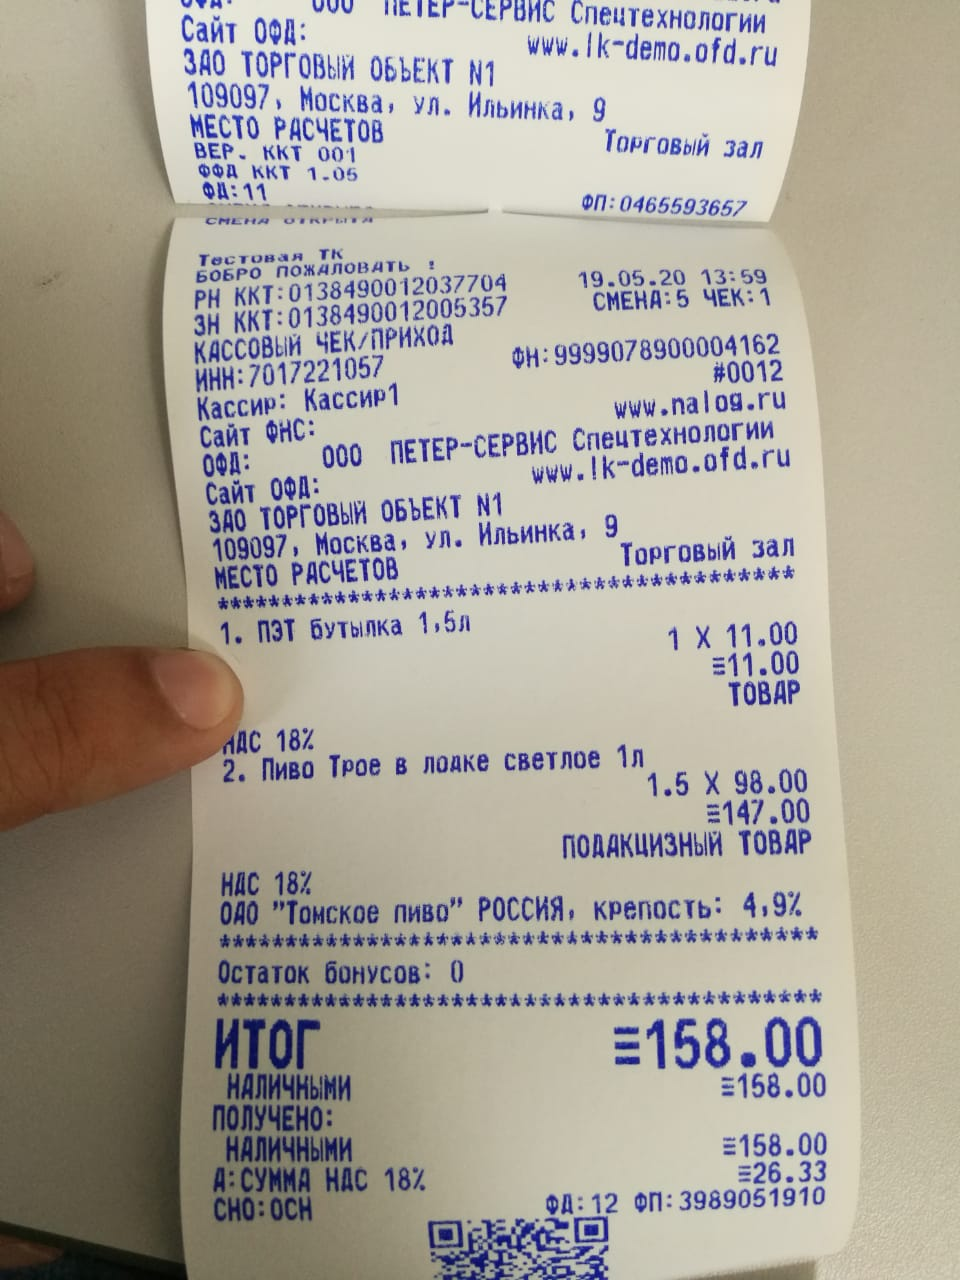
\includegraphics[width=125pt]{1.jpeg}} at (0pt,0pt)
\end{tikzpicture}
;\par
3. Поле <<СНО>> в чеке имеет значение <<ОСН>>;\par
4. Второй чек вида:
\begin{tikzpicture}
\pgftext{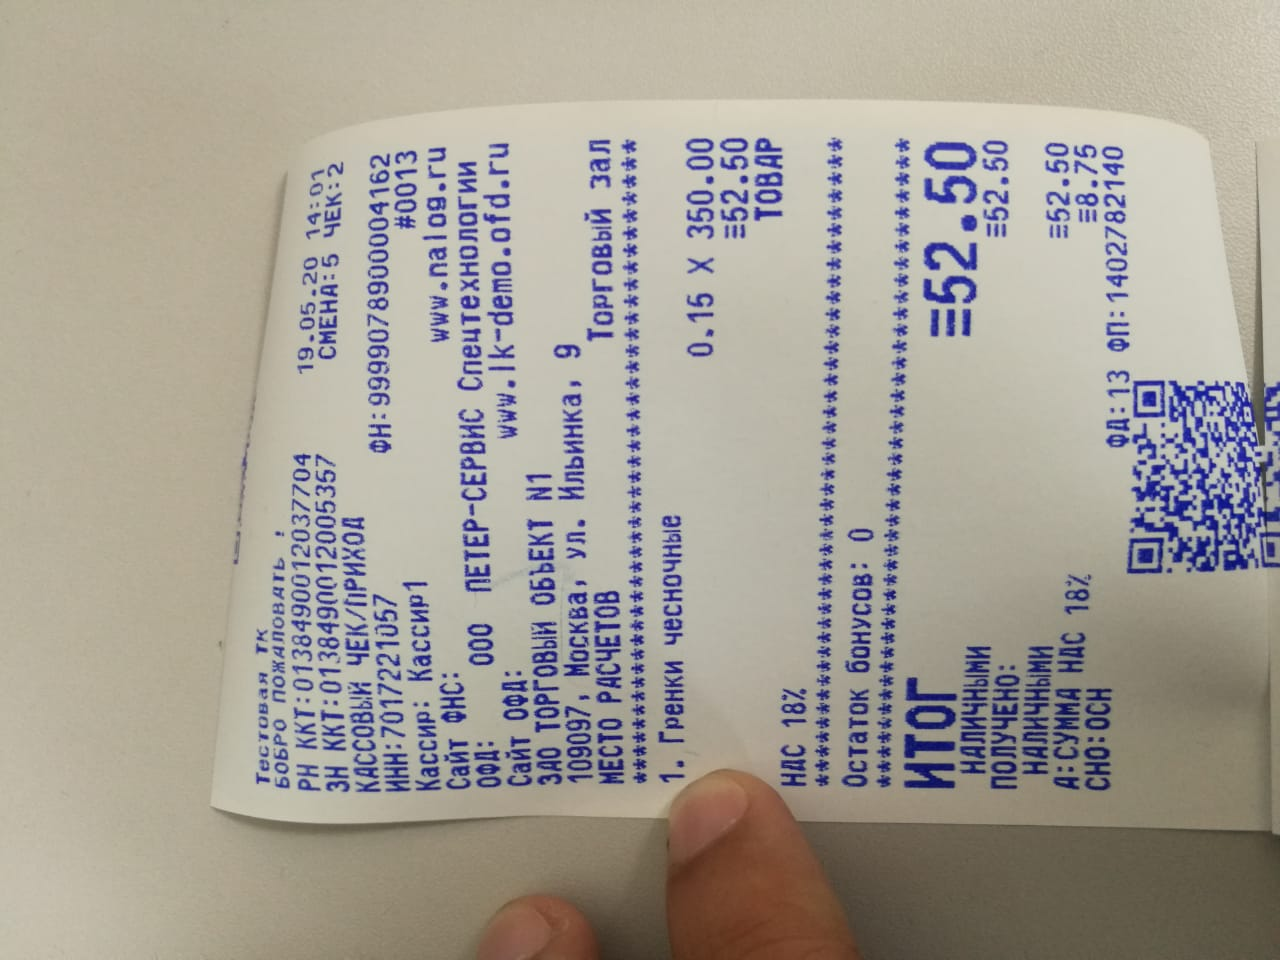
\includegraphics[width=125pt]{4.jpeg}} at (0pt,0pt)
\end{tikzpicture}
;\par
5. Поле <<СНО>> в чеке имеет значение <<УСН>>;\par
6. Табличная часть <<Товары>> в форме рабочего места кассира очистится;\par
&  \\
\hline
%****************************************************************************************************



\end{longtable}